\documentclass{report}
    % General document formatting
    %\usepackage[margin=0.7in]{geometry}
    %\usepackage[parfill]{parskip}
    \usepackage[utf8]{inputenc}
    
    % Related to math
    \usepackage{amsmath,amssymb,amsfonts,amsthm}
    
    \usepackage[french]{babel}
    \usepackage{hyperref}
    
    \usepackage{graphicx}
    \usepackage{float}
	\graphicspath{ {./images/} }
	
	\usepackage{xcolor}
	
	\usepackage{listings}
	\lstset{
	  basicstyle=\ttfamily,
	  columns=fullflexible,
	  frame=single,
	  breaklines=true,
	  postbreak=\mbox{\textcolor{red}{$\hookrightarrow$}\space},
	}
	
	\usepackage{csvsimple}
	\usepackage{multicol}
	\setlength{\columnsep}{1cm}
	
	\usepackage[useregional]{datetime2}
    
\title{
{Rapport sur le processus de calcul de la valeur moyenne de concentration de radon dans les bâtiments suisses}\\
{\large Office fédéral de la santé publique (OFSP)}\\
%{\includegraphics{university.jpg}}
}
\author{Niels Lachat}
\date{\today}

\newcommand{\bqmc}{$[Bq/m^3]$}

\begin{document}

\maketitle

\tableofcontents

\chapter{Introduction}
\section{But du document}
Le but de ce document est de décrire le processus de traitement de données utilisé pour calculer la valeur moyenne de concentration de radon dans les bâtiments suisses à partir des données de la base de données nationale de mesures du radon. 

\textit{Note}: Le code source du programme servant à effectuer ce calcul doit être mis à disposition avec ce document pour que le lecteur puisse s'y référer si besoin.

\section{Remarques}
Veuillez prendre compte des remarques suivantes lors de la lecture de ce document:
\begin{itemize}
\item Sauf indication contraire, toutes les dates sont données au format ISO-8601\footnote{\url{https://fr.wikipedia.org/wiki/ISO_8601}}.
\item Sauf indication contraire, les chemins d'accès faisant référence à des dossiers ou des fichiers du code source sont donnés depuis la racine du projet.
\end{itemize}

\section{Abbréviation utilisées dans le document}
Afin d'améliorer la lisibilité du document, nous utiliserons les abbréviations suivantes:

\begin{itemize}
\item \textbf{OFS} Office fédéral de la statistique
\item \textbf{BDD} Base de données
\end{itemize}

\section{Technologies utilisées pour le traitement de données}
Le programme effectuant le traitement de données et autres calculs est écrit dans le langage de programmation Scala (2.12.15)\footnote{\url{https://www.scala-lang.org/}}. La librairie utilisée pour faciliter les opérations sur des grands ensembles de données est Apache Spark (3.1.2) \footnote{\url{https://spark.apache.org/docs/3.1.2/}}. 

Pour simplifier l'importation des données dans le programme, l'outil OpenRefine (3.5.0) \footnote{\url{https://openrefine.org/}} a été utilisé pour prétraiter les données (voir chapitre \ref{chapterImportationEtPretraitement}).

\section{Référence pour la méthode de calcul}\label{sectionReferenceCalcul}
Le calcul décrit dans le présent document est basé sur le calcul de la valeur moyenne de concentration du radon effectué en 2004. Le document de référence se nomme "Strahlenexposition Bevölkerung 2004" et la section d'intérêt est la section 2 "Beitrag von Radon". 

Dans ce document, le calcul est effectué en 3 étapes.
\subsection{Correction pour la saison}
La moyenne de concentration doit être calculée en considérant une moyenne annuelle, en prenant en compte que les séjours à l'intérieur sont plus longs en hiver qu'en été. Cette correction a déjà été appliquée au moment où les mesures sont entrées dans la BDD radon. 

Pour refléter cette correction dans la notation (et pour garder la même notation que dans le document de référence), nous considérerons que $A_0$ représente la valeur mesurée de concentration de radon en \bqmc, corrigée pour représenter une moyenne annuelle.

\subsection{Correction pour l'étage} \label{introCorrectionEtage}
Pour mieux refléter la concentration de radon dans laquelle la population vit, une correction a été appliquée lors du calcul de 2004. Les valeurs mesurées au-dessous de l'étage moyen d'habitation des bâtiments du canton sont attenuées, et les valeurs mesurées au-dessus sont accentuées. La formule de correction est la suivante:

\begin{equation}\label{formuleCorrectionEtage}
A_{0,St} = A_0 \cdot e^{-0.19 \cdot (St_m - St)}
\end{equation}

où

\begin{itemize}
\item $A_{0,St}$ représente la concentration corrigée pour l'étage, en \bqmc
\item $A_0$ représente la concentration avant correction, en \bqmc
\item $e^x$ représente la fonction exponentielle évaluée en $x$
\item $St_m$ L'étage moyen d'habitation dans le canton où la mesure a été effectuée, $\in \mathbb{R}$
\item $St$ L'étage auquel la mesure a été effectuée, $\in \mathbb{Z}$
\end{itemize}

\subsection{Calcul final de la concentration moyenne suisse}
Le calcul final de la concentration moyenne de radon dans les locaux d'habitation et de séjour est calculée comme suit:

\begin{equation}\label{formuleCalculFinalConcentration}
A = \frac{1}{\sum_{i=1}^{N} pop_i} \sum_{i=1}^{N} pop_i [ \frac{1}{N_i} \sum_{j=1}^{N_i} [\frac{1}{N_{ij}} \sum_{k=1}^{N_{ij}} A_{0, St_{ijk}}] ]
\end{equation}

où

\begin{itemize}
\item $A$ représente la concentration moyenne de radon finale, en \bqmc
\item $pop_i$ représente la population de la commune $i$
\item $N$ représente le nombre total de communes pour lesquelles des mesures existent
\item $N_i$ représente le nombre de bâtiments mesurés dans la commune $i$
\item $N_{ij}$ représente le nombre de mesures effectuées dans le bâtiment $j$ de la commune $i$
\item $A_{0, St_{ijk}}$ représente la $k$-ème mesure, corrigée pour l'étage, effectuée dans le bâtiment $j$ de la commune $i$, en \bqmc
\end{itemize}


\section{Vue d'ensemble du processus de traitement de données}
Nous décrirons ici le processus du traitement des données, depuis les données brutes décrites dans le chapitre \ref{chapterSourcesDesDonnees}, jusqu'à l'obtention de la valeur moyenne de concentration de radon. Chaque étape du processus sera expliquée en détail dans les chapitres suivants.

\subsection{Importation et prétraitement}
Dans cette étape, les données brutes sont importées dans le programme et sont prétraitées pour les étapes suivantes.

\subsection{Filtration}
Dans cette étape, les données brutes prétraitées sont filtrées afin de supprimer les entrées invalides et les valeurs qu'on ne veut pas retenir pour le calcul final de la valeur moyenne (par exemple les mesures dans des locaux qui ne sont pas des locaux de séjour prolongé).

\subsection{Corrections}
Dans cette étape, les mesures brutes subissent une correction ou ajustement qui dépend de l'étage dans lequel la mesure a été prise. 

\subsection{Calcul de la valeur moyenne}
Finalement les données traitées sont utilisées pour calculer la concentration moyenne de radon dans les bâtiments suisses selon la méthode appliquée en 2004. 




\chapter{Sources des données}\label{chapterSourcesDesDonnees}
Dans ce chapitre, nous décrirons les sources des données utilisées pour le calcul de la valeur moyenne de concentration de radon.

\section{Base de données nationale du radon}
La source principale des données est la BDD nationale du radon. Cette BDD contient 279'257 entrées, une pour chaque mesure de radon effectuée.
Elle a été exportée initialement sous forme de fichier excel nommé "Messungen\_020721.xlsx". C'est ce fichier que nous considèreront comme la source initiale des données. % TODO est-ce qu'on peut référencer ces données de façon plus précise?

\begin{itemize}
\item \textbf{Période de récolte des données} [1982]-[2021] % TODO est-ce que c'est correct?
\item \textbf{Date de publication} 2021-07-02
\item \textbf{Lien vers les données} Données non disponibles publiquement
\end{itemize}

\section{Nombre d'étages des bâtiments par canton}\label{sectionCantonEtagesBatiments}
Afin d'effectuer la correction mentionnée au point \ref{introCorrectionEtage} il est nécessaire d'avoir des données concernant l'étage d'habitation moyen par canton. Malheureusement, cette information n'est pas disponible directement sur le catalogue de données de l'OFS. Ce qui est par contre disponible, c'est le nombre de bâtiments qui ont un certain nombre d'étages, par canton. Pour obtenir le fichier source dans le format que le programme accepte, il faut aller sur ce lien \url{https://www.pxweb.bfs.admin.ch/pxweb/fr/px-x-0902010000_101/px-x-0902010000_101/px-x-0902010000_101.px} et sélectionner les options comme dans la figure \ref{fig:nbFloorsBuildingExportOptions}. Il faut ensuite cliquer sur le bouton "Continuer" et enregistrer les données sous forme de fichier CSV.

\begin{figure}[H]
    \centering
    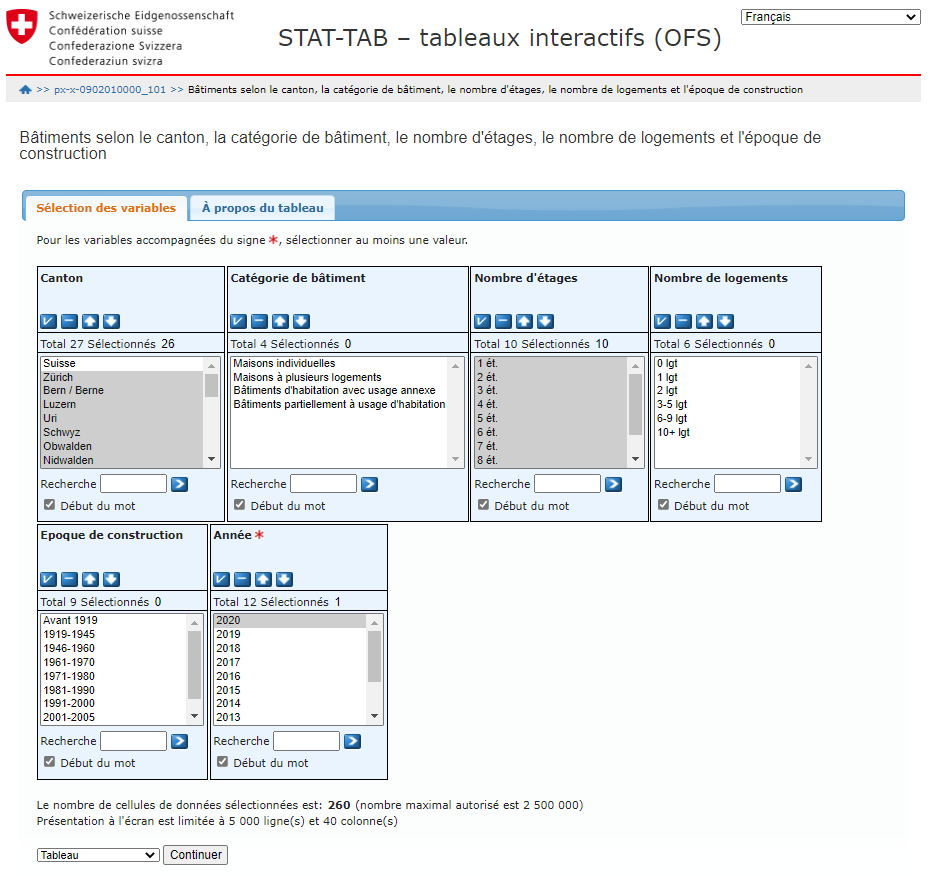
\includegraphics[width=\textwidth]{nb-floors-building-export-options}
    \caption{Options à sélectionner pour exporter les données du nombre d'étage des bâtiments par canton}
    \label{fig:nbFloorsBuildingExportOptions}
\end{figure}

Dans le chapitre \ref{chapterImportationEtPretraitement} nous expliquerons comment passer de ces données brutes à l'étage moyen d'habitation de la population, par canton.

\begin{itemize}
\item \textbf{Période de récolte des données} [2009]-[2020]
\item \textbf{Date de publication} 2021-10-07
\item \textbf{Lien vers les données} \url{https://www.bfs.admin.ch/bfs/fr/home/statistiques/construction-logement/batiments.assetdetail.19024696.html}
\end{itemize}


\section{Nombre d'habitants par commune}\label{sectionNombreHabitantsCommunes}
La moyenne de concentration est pondérée pour chaque commune par le nombre d'habitants dans la commune. Il est donc nécessaire d'avoir la population de chaque commune suisse. 

\begin{itemize}
\item \textbf{Période de récolte des données} [2004]-[2020]
\item \textbf{Date de publication} 2021-03-26
\item \textbf{Lien vers les données} \url{https://www.bfs.admin.ch/bfs/fr/home/statistiques/statistique-regions/portraits-regionaux-chiffres-cles/communes.assetdetail.15864461.html}
\end{itemize} 

\chapter{Importation et prétraitement (preprocessing)}\label{chapterImportationEtPretraitement}
\section{BDD radon}

\subsection{Importation}

\subsubsection{Transformation du fichier xlsx en csv}
A partir du fichier source au format \textit{xlsx}, nous utilisons le programme Excel 2016 pour exporter les données dans un format plus facile à traiter par OpenRefine. Lorsque le fichier est ouvert avec Excel 2016, il faut suivre les étapes suivantes: Fichier $>$ Exporter $>$ Modifier le type de fichier $>$ CSV (séparateur: point-virgule) (*.csv) $>$ Enregistrer sous.

\subsubsection{Nettoyage par OpenRefine}
Nous devons à présent passer le fichier par OpenRefine afin d'éliminer des colonnes inutiles et de transformer les données dans un format acceptable par notre programme. Pour ce faire, il faut créer un nouveau projet OpenRefine à partir du fichier csv crée précedemment, puis l'exporter en appliquant les options d'exportation trouvable dans la source du programme sous "metadata/rn-db\_openrefine-options.json". Une chose à ne pas oublier lors de cette étape est de cocher la case "Ignore facets and filters and export all rows" afin d'exporter toutes les lignes du fichier.

Le fichier ainsi généré doit être placé sous "data/rn-db/main.csv"

\subsection{Prétraitement}

La BDD radon ne nécessite pas de prétraitement avant de pouvoir être utilisée par le programme. Il faut cependant que les dates de début et de fin de la mesure du radon (colonnes START\_TIME et END\_TIME) soient transformées au format ISO 8601. La transformation de la date est faite par Spark en lui fournissant comme option d'importation "dateFormat" $\rightarrow$ "dd.MM.yyyy". 

Pour connaître les champs de la BDD qui sont utilisés dans le programme, voir "src/main/scala/data/RadonDatabase.scala" (voir annexe \ref{sectionRadonDatabaseScala}). 

\section{Étage moyen d'habitation}

\subsection{Importation}
Nous transformons le fichier téléchargé à la section \ref{sectionCantonEtagesBatiments} à l'aide d'OpenRefine. Les options par défault peuvent être gardées pour créer le projet OpenRefine. Il faut ensuite utiliser les options d'exportation trouvables dans le fichier suivant: "metadata/canton-floors-buildings\_openrefine-options.json" pour exporter le fichier traité.

Le fichier ainsi généré doit être placé sous "data/avg-floor/2020/main.csv"

\subsection{Prétraitement}

Pour plus de détails sur les opérations décrites dans cette section, veuillez vous référer à "src/main/scala/data/AverageFloor2020.scala" (voir annexe \ref{sectionAverageFloor2020Scala}). 
\subsubsection{Conversion des colonnes en format utile}
Les colonnes "Canton" et "Nombre d'étages" doivent être traitées avant de pouvoir être utilisées car elles ont un format non compatible avec les autres sources de données. 
\begin{itemize}
\item Pour la colonne "Canton", chaque nom de canton écrit en toutes lettres est converti dans le code à 2 lettres du canton (exemple "Bern / Berne" $\rightarrow$ "BE")
\item Pour la colonne "Nombre d'étages", chaque description du nombre d'étages est converti en un nombre simple (exemple "4 ét." $\rightarrow$ 4, "10+ ét." $\rightarrow$ 10\footnote{On notera d'ailleurs ici qu'une partie du sens des données initiales est perdu comme on considère que tous les bâtiments qui ont \textbf{plus de} 10 étages ont \textbf{exactement} 10 étages. Cette simplification ne devrait cependant pas avoir un impact significatif sur le résultat comme la majorité des bâtiments en Suisse ont moins de 10 étages (ceci est visible facilement dans les données du nombre d'étage des bâtiments par canton).})
\end{itemize}

\subsubsection{Calcul de l'étage d'habitation moyen par canton}\label{importationEtageMoyen}
Pour calculer l'étage moyen d'habitation par canton, nous utilisons la moyenne pondérée du nombre d'étages par le nombre de bâtiments qui ont ce nombre d'étages:

\begin{equation}
E_c = \frac{1}{2} \cdot \frac{\sum_{e=1}^{10} n_{e,c} \cdot e}{\sum_{e=1}^{10} n_{e,c}}
\end{equation}

où

\begin{itemize}
\item $E_c$ représente l'étage moyen d'habitation dans le canton $c$
\item $n_{e,c}$ représente le nombre de bâtiments qui ont $e$ étages dans le canton $c$
\end{itemize}

Il est très important de noter ici qu'il faut distinguer le \textbf{nombre} d'étages, et l'étage moyen \textbf{d'habitation}. C'est pour cette raison que nous multiplions la moyenne pondérée du \textbf{nombre} d'étages par un facteur $\frac{1}{2}$. Nous pouvons en effet observer que par exemple, pour un bâtiment de 5 étages, les habitants résident en moyenne à l'étage 2.5 (en supposant que tous les étages sont uniformément occupés).

Ci-dessous, nous montrons les valeurs de l'étage moyen d'habitation par canton, en 2004, 2009 et 2020. Les données de 2004 sont issues du document cité à la section \ref{sectionReferenceCalcul}. Les données pour 2009 et 2020 sont calculées à partir du nombre d'étages par bâtiment (données de l'OFS). Les valeurs pour 2004 et 2009 sont données comme points de comparaison avec les valeurs de 2020 qui sont utilisées pour le calcul de la valeur moyenne de la concentration de radon. 
Il est important de noter ici, que les différences entre les valeurs de 2004 et 2009 sont plus importantes qu'entre 2009 et 2020. Un exemple frappant est la valeur pour le canton de Genève qui passe de 2.89 en 2004 à 1.67 en 2009 et reste à 1.67 en 2020. Ceci nous laisse à penser qu'il y a une différence dans la méthode de calcul ou dans la source des données entre ce qui avait été calculé en 2004 et ce que nous avons calculé pour 2009 et 2020. Cependant il nous est impossible d'être certain d'où vient la différence car le rapport de 2004 est imprécis sur la source de ces données. La seule indication qui nous est donnée est: "Quelle: Bundesamt für Statistik" (en français: "Source: Office fédéral de la statistique"). 
Nous considérons cependant que notre source de données et notre méthode de calcul semblent correctes et nous utiliserons donc les valeurs d'étage moyen d'habitation pour 2020 que nous avons calculées pour la suite des calculs.
\pagebreak

\begin{center}
\begin{multicols}{3}[Étage moyen d'habitation, en 2004, en 2009 et en 2020 respectivement]
\csvautotabular{../data/avg-floor/2004/avg-floor-per-canton-2004-COMMA_CSV.csv}
\csvautotabular{../data/avg-floor/2009/computed-avg/kanton-etage.csv}
\csvautotabular{../data/avg-floor/2020/computed-avg/kanton-etage.csv}
\end{multicols}
\end{center}

\section{Nombre d'habitants par commune}
\subsection{Importation}

À partir du fichier \textit{xlsx} téléchargé à la section \ref{sectionNombreHabitantsCommunes}, nous utilisons OpenRefine pour transformer les données dans un format traitable par notre programme.

Les options d'importation pour OpenRefine doivent être ajustées pour traiter correctement le fichier \textit{xlsx} qui a une structure peu régulière. Veuillez vous référer à la figure \ref{fig:importPopulationPerTownOpenRefine}.

\begin{figure}[H]
    \centering
    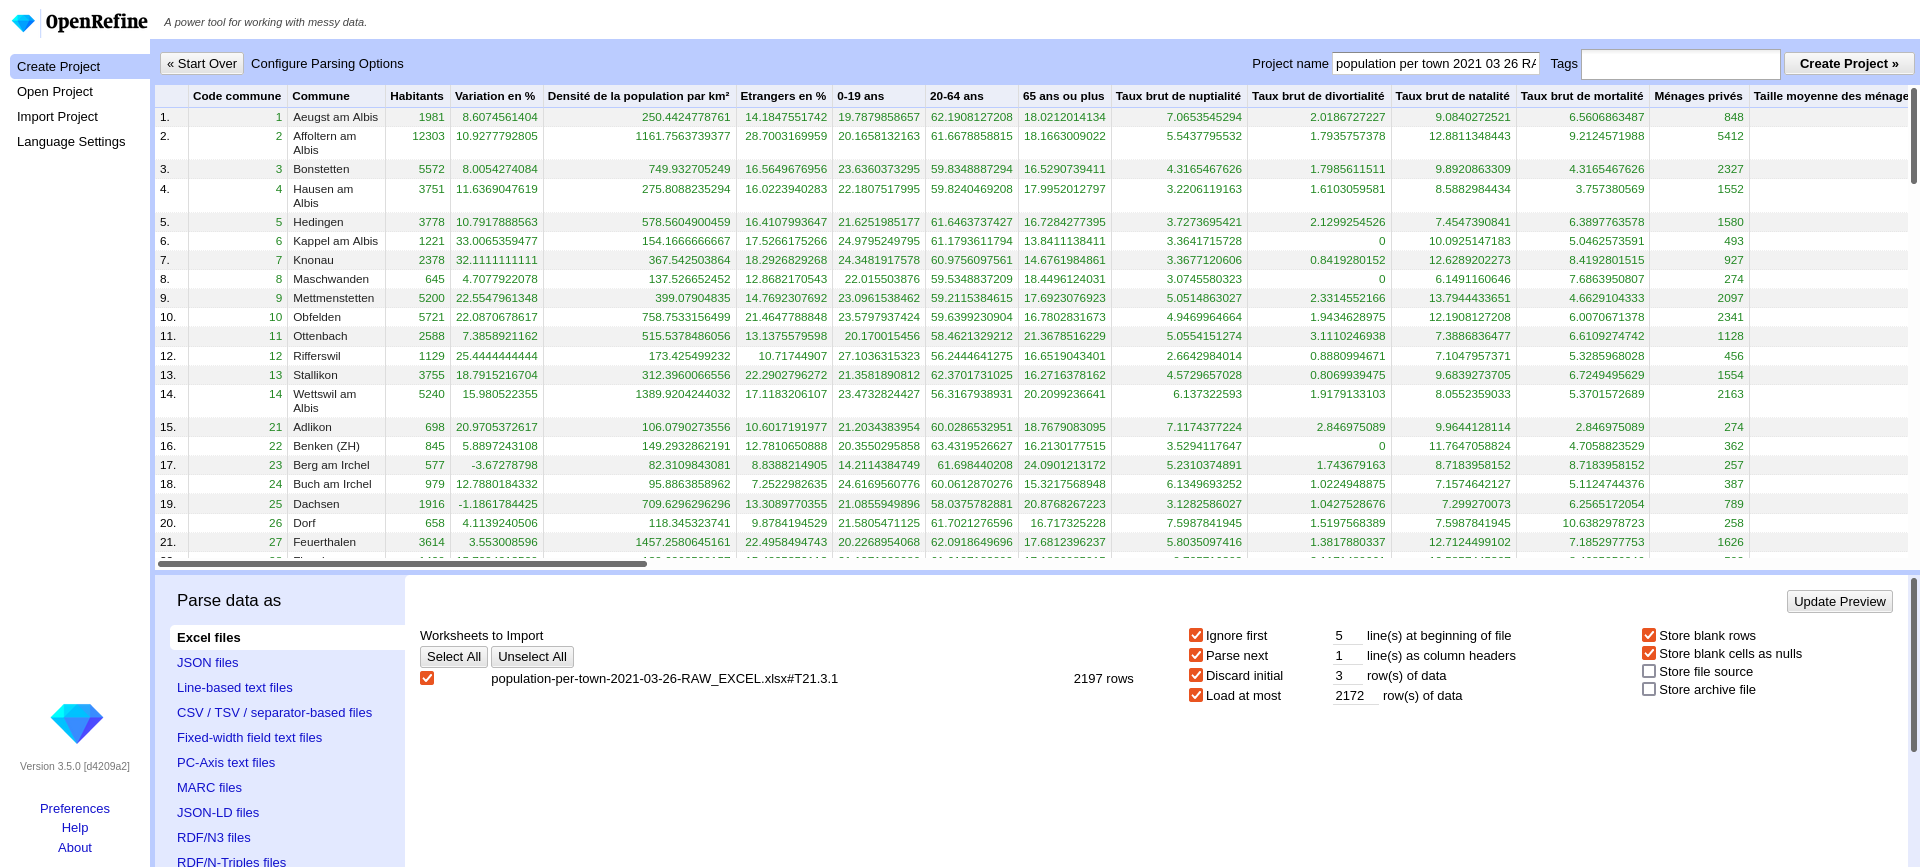
\includegraphics[width=\textwidth]{import-population-per-town-OPENREFINE}
    \caption{Options à sélectionner pour créer le projet OpenRefine. Ignore first = 5, Parse next = 1, Discard initial = 3, Load at most = 2172}
    \label{fig:importPopulationPerTownOpenRefine}
\end{figure}

Il faut ensuite utiliser les options d'exportation trouvables dans le fichier suivant: "metadata/population-per-town\_openrefine-options.json" pour exporter le fichier traité.

Le fichier ainsi généré doit être placé sous "data/population-per-town/main.csv".

\subsection{Prétraitement}
Le seul prétraitement qui doit être effectué est de convertir les nombres (numéro de commune et population correspondante) d'un type de nombre réel (avec des $.0$ en suffixe) en nombre entier. Ceci est fait dans "src/main/scala/data/TownPopulations.scala".

\chapter{Filtration}
\newcommand{\nbEntreesAvantFiltration}{279'257}
\newcommand{\nbEntreesApresFiltration}{168'056}
\newcommand{\nbEntreesSupprParFiltration}{111'201}


\newcommand\filterProps[2]{
\begin{table}[H]
\centering
\begin{tabular}{|l|l|}
\hline
%Propriété                          & Valeur \\ \hline
Nombre maximal d'entrées supprimées & #1   \\ \hline
Pourcentage maximal d'entrées supprimées & #2\% \\ \hline
\end{tabular}
\end{table}
}


Dans ce chapitre nous décrirons les différents filtres qui sont appliqués à la BDD radon dans le but d'éliminer les mesures invalides et les mesures qui ne correspondent pas aux critères du calcul (locaux non habités).

Pour plus de détails concernant le processus de filtration, veuillez vous référer au fichier "src/main/scala/v01/Filtering.scala" (voir \ref{sectionAverageFloor2020Scala}).

\textit{Note}: Pour chaque filtre on compte le nombre d'entrées maximal que ce filtre peut supprimer, et quel pourcentage du nombre d'entrées initial cela représente. Ceci permet d'observer quels filtres auront le plus grand impact sur le calcul final. Ceci est montré comme suit:
\filterProps{$N$}{$P$}

Où
\begin{itemize}
\item $N$ représente le nombre d'entrées maximal que ce filtre peut supprimer
\item $P$ représente le pourcentage du total initial d'entrées. $P = N / \nbEntreesAvantFiltration $
\end{itemize}

\section{Conserver uniquement les mesures valides}
Ce filtre conserve uniquement les entrées où la colonne VALIDIERUNG vaut "Y".

\filterProps{11'781}{4.22}

%\section{Exclure les mesures de locaux inhabités}\label{filter:RAUMTYP}
%Ce filtre supprime les entrées où la colonne RAUMTYP vaut "Keller", "K" ou "?"\footnote{Les entrées avec "?" ont été supprimées par mesure de précaution, pour éviter d'inclure des mesures indésirables.}

%\filterProps{62'314}

\section{Conserver uniquement les locaux avec séjour de personnes}\label{filter:PERSONENAUFENTHALT}
Ce filtre conserve uniquement les entrées où la colonne PERSONENAUFENTHALT vaut "YES\_LONG" ou "YES\_SHORT"

\filterProps{79'358}{28.42}

\section{Conserver uniquement les entrées qui contiennent une mesure}
Ce filtre conserve uniquement les entrées qui contiennent une valeur dans la colonne RADONKONZENTRATION\_BQ\_M3.

\filterProps{6'486}{2.32}

\section{Exclure les mesures effectuées dans des communes qui n'existent plus}
Après inspection des données, il s'est avéré que certaines mesures ont été effectuées dans des communes qui n'existent plus dans les données de population de l'OFS (voir \ref{sectionNombreHabitantsCommunes}). Cela est probablement dû principalement à des fusions de communes. Il serait techniquement possible de trouver les communes qui ont fusionné et remplacer les anciens numéros de communes par les nouveaux numéros de communes fusionnées, mais cela serait relativement couteux en terme de temps. C'est pourquoi il a été décidé d'ignorer les mesures effectuées dans ces communes "disparues".

Ce filtre fonctionne en plusieurs étapes:
\subsection{Trouver les numéros des communes disparues}
Pour ce faire, nous collectons l'ensemble des numéros de communes qui apparaissent dans la BDD radon (colonne GEMEINDENUMMER), nommons cet ensemble $C_{Rn}$. Nous collectons ensuite l'ensemble des numéros de communes qui apparaissent dans le tableau des populations des communes (voir \ref{sectionNombreHabitantsCommunes}), nommons cet ensemble $C_{Pop}$. 

Les numéros des communes disparues sont donnés par la différence entre les ensembles: 
\begin{equation}
D = C_{Rn} - C_{Pop}
\end{equation}

Pour les données que nous utilisons, $|D| = 60$.

Pour plus de détails concernant cette étape, voir "src/main/scala/main/DataExploration.scala".

\subsection{Conserver uniquement les mesures effectuées dans les communes non disparues}
Nous conservons ensuite uniquement les mesures qui ont été effectuées dans une commune qui n'apparait pas dans $D$.

\filterProps{5'078}{1.82}

\section{Garder uniquement les mesures effectuées dans les étages entre 0 et 20}\label{filter:ETAGE}
Afin d'inclure uniquement les locaux d'habitation dans le calcul de la valeur moyenne de concentration, nous gardons uniquement les entrées où 
\begin{equation}
0 \leq ETAGE \leq 20
\end{equation}

\filterProps{73'059}{26.16}

\section{Exclure les mesures effectuées avant un assainissement radon}\label{filter:SANIERUNG}
Pour les bâtiments qui ont subit un assainissement radon, des mesures ont été effectuées \textit{avant} et \textit{après} assainissement. Afin de représenter plus précisement la valeur de concentration de radon réelle, il faut exclure les mesures effectuées avant assainissement des mesures considérées pour le calcul de la valeur moyenne de concentration.

Ceci se fait en plusieurs étapes:
\subsection{Trouver les identifiants des mesures effectuées avant assainissement}
Dans cette étape, nous trouvons les identifiants des mesures (ID\_MESSUNG) effectuées avant assainissement (dans les cas où il existe des mesures avant et après assainissement pour un bâtiment donné). Appelons cette liste d'identifiants $L$.

La méthode pour effectuer cette opération est la suivante:
\begin{enumerate}
\item Grouper les entrées par bâtiment (à l'aide de la colonne ID\_HAUS)
\item Pour chaque bâtiment on trouve s'il y a eu un assainissement (si pour le bâtiment en question, une des entrées a MESSTYP = "Messung nach der Sanierung", on considère qu'il y a eu assainissement)
\item Si c'est le cas, on ajoute tous les identifiants des mesures effectuées avant assainissement dans le bâtiment à $L$ (l'identifiant de toutes les entrées où MESSTYP = "Messung" pour le bâtiment). Autrement, $L$ reste inchangée.
\end{enumerate}

Pour plus de détails, voir "src/main/scala/v01/Filtering.scala:findIdsOfMeasurementsBeforeRemediation".

\subsection{Exclure les mesures effectuées avant assainissement}
Cette étape est relativement simple une fois qu'on a obtenu $L$. Il suffit de supprimer les mesures dont l'identifiant se trouve dans $L$.

\filterProps{5'623}{2.01}

\section{Exclure les mesures de concentration = 0 \bqmc}
La BDD contient des entrées où RADONKONZENTRATION\_BQ\_M3 vaut 0, et il est impossible qu'un appareil de mesure correctement utilisé mesure une moyenne de 0 \bqmc. Il faut donc exclure ces mesures du calcul final. 
Par mesure de précaution, le filtre conserve uniquement les mesures $> 0$ \bqmc et supprime donc aussi d'éventuelles valeurs négatives de concentration.

\filterProps{1'678}{0.60}

\section{Conclusion}

Après filtration, la BDD radon est réduite à \nbEntreesApresFiltration\ entrées. À l'origine, elle contenait \nbEntreesAvantFiltration\ entrées. L'étape de filtration supprime donc \nbEntreesSupprParFiltration\ entrées.

Il faut noter que le nombre d'entrées supprimées ne correspond pas à la somme du nombre maximal d'entrées supprimées par chaque filtre, car certaines entrées sont exclues par plusieurs filtres à la fois (par exemple une mesure dans une cave effectuée avant un assainissement sera supprimée à cause des filtres décrits en \ref{filter:PERSONENAUFENTHALT}, \ref{filter:ETAGE}, \ref{filter:SANIERUNG}). 


\chapter{Corrections}
Après filtration, les mesures doivent encore être corrigées en fonction de l'étage auquel elles ont été mesurées (comme expliqué dans la section \ref{introCorrectionEtage}).

Nous décrirons ici les étapes qui permettent de corriger les mesures en fonction de l'étage.
Pour chaque entrée, il faut:
\begin{enumerate}
\item Récupérer le canton dans lequel la mesure a été effectuée (colonne KANTON)
\item Trouver l'étage d'habitation moyen du canton grâce aux données importées à la section \ref{importationEtageMoyen} (valeur $St_m$)
\item Récupérer l'étage auquel la mesure a été effectué (colonne ETAGE $\rightarrow$ valeur $St$)
\item Récupérer la valeur mesurée de concentration (colonne RADONKONZENTRATION\_BQ\_M3 $\rightarrow$ valeur $A_0$)
\item Calculer la valeur corrigée de concentration grâce à la formule \ref{formuleCorrectionEtage}
\end{enumerate}

Pour plus de détail, veuillez vous référer à "src/main/scala/v01/Corrections.scala" (voir \ref{sectionCorrectionsScala})

\chapter{Calcul de la valeur moyenne}
Dans ce chapitre, nous décrirons la façon dont est calculée la valeur moyenne à partir de la BDD radon filtrée et corrigée et des autres données nécessaires.

Le calcul s'effectue en plusieurs étapes que nous détaillerons ici.
Chaque étape représente une partie de la formule \ref{formuleCalculFinalConcentration}.

Pour plus de détails, veuillez vous référer à "src/main/scala/v01/ComputeAverageVolumetricActivity.scala" (voir \ref{sectionComputeAverageVolumetricActivityScala})

\section{Calcul de la moyenne de concentration par bâtiment}
Nous commençons par calculer la moyenne de concentration de radon par bâtiment, selon la formule suivante (moyenne arithmétique des valeurs mesurées dans le bâtiment $j$ de la commune $i$):

\begin{equation}
A_{ij} = \frac{1}{N_{ij}} \sum_{k=1}^{N_{ij}} A_{0, St_{ijk}}
\end{equation}

où
\begin{itemize}
\item $A_{ij}$ représente la concentration moyenne de radon dans le bâtiment $j$ de la commune $i$, en \bqmc
\item $N_{ij}$ représente le nombre de mesures effectuées dans le bâtiment $j$ de la commune $i$
\item $A_{0, St_{ijk}}$ représente la $k$-ème mesure, corrigée pour l'étage, effectuée dans le bâtiment $j$ de la commune $i$, en \bqmc
\end{itemize}

Concrètement, ce calcul se fait en groupant les entrées par ID\_HAUS et en calculant la moyenne pour chaque groupe.

\section{Calcul de la moyenne de concentration par commune}
Cette étape est très similaire à l'étape précédente. Nous décrirons donc uniquement la formule nécessaire au calcul.

\begin{equation}
A_i = \frac{1}{N_i} \sum_{j=1}^{N_i} A_{ij} 
\end{equation}

où 
\begin{itemize}
\item $A_i$ représente la concentration moyenne de radon dans la commune $i$, en \bqmc
\item $N_i$ représente le nombre de bâtiments mesurés dans la commune $i$
\item $A_{ij}$ représente la concentration moyenne de radon dans le bâtiment $j$ de la commune $i$, en \bqmc
\end{itemize}

\section{Calcul final de la concentration moyenne suisse}
Finalement, dans cette étape nous calculons la valeur moyenne de concentration de radon dans les bâtiments suisses. La formule est une moyenne pondérée des concentrations des communes par les populations des communes.

\begin{equation}
A = \frac{1}{\sum_{i=1}^{N} pop_i} \sum_{i=1}^{N} pop_i \cdot A_i
\end{equation}

où
\begin{itemize}
\item $A$ représente la valeur moyenne de concentration de radon dans les bâtiments suisses, en \bqmc
\item $pop_i$ représente la population de la commune $i$
\item $N$ représente le nombre total de communes pour lesquelles des mesures existent
\item $A_i$ représente la concentration moyenne de radon dans la commune $i$, en \bqmc
\end{itemize}

D'un point de vue du programme, on commence par calculer la somme du produit de la population par la concentration de la commune, puis on divise par la population totale \textbf{des communes dans lesquelles des mesures ont été effectuées.} (pour plus de détails voir \ref{sectionComputeAverageVolumetricActivityScala})

\chapter{Conclusion}
En conclusion, nous avons pu reproduire le calcul de la valeur moyenne de radon dans le bâtiments suisses de la même façon qu'elle avait été calculée en 2004. 

Il pourrait également être intéressant de comparer ce résultat avec d'autres méthodes de calcul (ajustement avec une distribution normale, utilisation d'autres fonctions que la moyenne pour calculer une valeur représentative d'un bâtiment (maximum des mesures, moyenne géométrique des mesures)). Ceci pourra être effectué dans un second temps.

\chapter{Annexes}
\UseRawInputEncoding

\section{RadonDatabase.scala}\label{sectionRadonDatabaseScala}
\lstinputlisting[language=Scala]{../src/main/scala/data/RadonDatabase.scala}

\section{AverageFloor2020.scala}\label{sectionAverageFloor2020Scala}
\lstinputlisting[language=Scala]{../src/main/scala/data/AverageFloor2020.scala}

\section{Filtering.scala}\label{sectionFilteringScala}
\lstinputlisting[language=Scala]{../src/main/scala/data_processing/Filtering.scala}

\section{Corrections.scala}\label{sectionCorrectionsScala}
\lstinputlisting[language=Scala]{../src/main/scala/data_processing/Corrections.scala}

\section{ComputeAverageVolumetricActivity.scala}\label{sectionComputeAverageVolumetricActivityScala}
\lstinputlisting[language=Scala]{../src/main/scala/v01/ComputeAverageVolumetricActivity.scala}

\end{document}